To estimate real-time joints kinematics and muscles activations which are dynamically consistent, bioptim was used to implement a moving horizon estimation (MHE). 
The example is given for a shoulder elevation motion using a 4-DoFs arm actuated by 19 Hill-type muscles.
Muscle activations were the controls of the OCP.
The OCP was split into a succession of smaller one. Each objective function (Eq.~\ref{eq:ocp_exMHE}) was written as the sum of three terms: first correspond to tracking reference joint angles, second and third correspond to states and muscle activation regularization (i.e., least-square criteria): 

\[ 
\resizebox{0.9\columnwidth}{!}{$ 
\begin{aligned}
\mathcal{J} = \sum_{n}^{n + n_{mhe}}\underbrace{\omega_1´(\|q_{ref} - q_{est}\|^{2})}_{TRACK\_STATE} ~  
+ ~ \underbrace{\omega_2\int_t^{t+t_{mhe}} \sum_{i=1}^{8}~ q_{est_i}^2~dt}_{MINIMIZE\_ STATE} ~  
+ ~ \underbrace{\omega_3\int_t^{t+t_{mhe}} \sum_{i=1}^{19}~U_{i}^2~dt}_{MINIMIZE\_ ACTIVATION}, 
\end{aligned}  
$}  
\addtag  
\label{eq:ocp_exMHE}  
\]  

\noindent where $\omega_1$ =1e4, $\omega_2$ = 10, $\omega_3$ = 100, $n_{mhe}=7$ is the number of OCP shooting nodes and $t_{mhe}$ is OCP duration. $q_{ref}$, $q_{est}$ and $U_i$ are respectively reference and estimate joints angles, and muscles activations. 

In this example, reference data of an 8 s series of 4 arm elevations were generated at 100~Hz, by computer simulation, with co-activation on two antagonists muscles groups (triceps and biceps).
Since successive problems are highly similar, due to the MHE, a warm-start strategy based on the previous solutions was implemented.

Using a windows size of 7 nodes, the estimator ran at about 50~Hz (one in two reference data frame was sent to the estimator to correspond with experimental conditions), i.e. four times faster than standard biofeedback (13~Hz, \cite{kannape2013biofeedback}).
The estimator was able to forecast the movement kinematic (Fig.~\ref{fig:joints_angles_MHE}) with a consistent dynamics and a root mean square error of $0.02\pm6e\emph{-3}\text{~}^{\circ}$.
Due to co-contraction, the estimated muscles activations were lower than reference activations but with a similar pattern (Fig.~\ref{fig:muscles_excitations_MHE}).  

 

\begin{figure*}[t!] 
\centering 
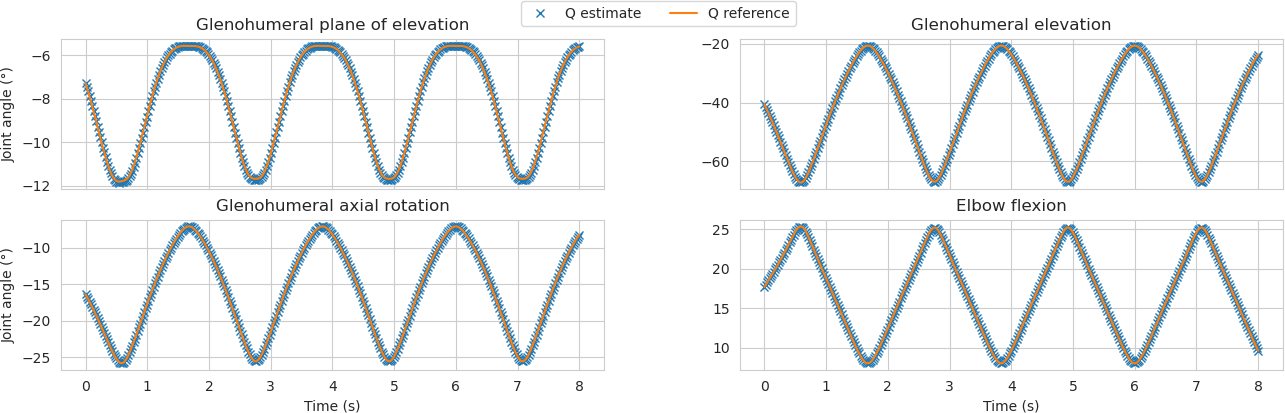
\includegraphics[width=\textwidth]{Articular_angle_MHE.png}\\ 
\caption{Time histories of estimate joints angles (blue cross) and reference joints angles (orange line).} 
\label{fig:joints_angles_MHE} 
\end{figure*} 

\begin{figure*}[t!] 
\centering 
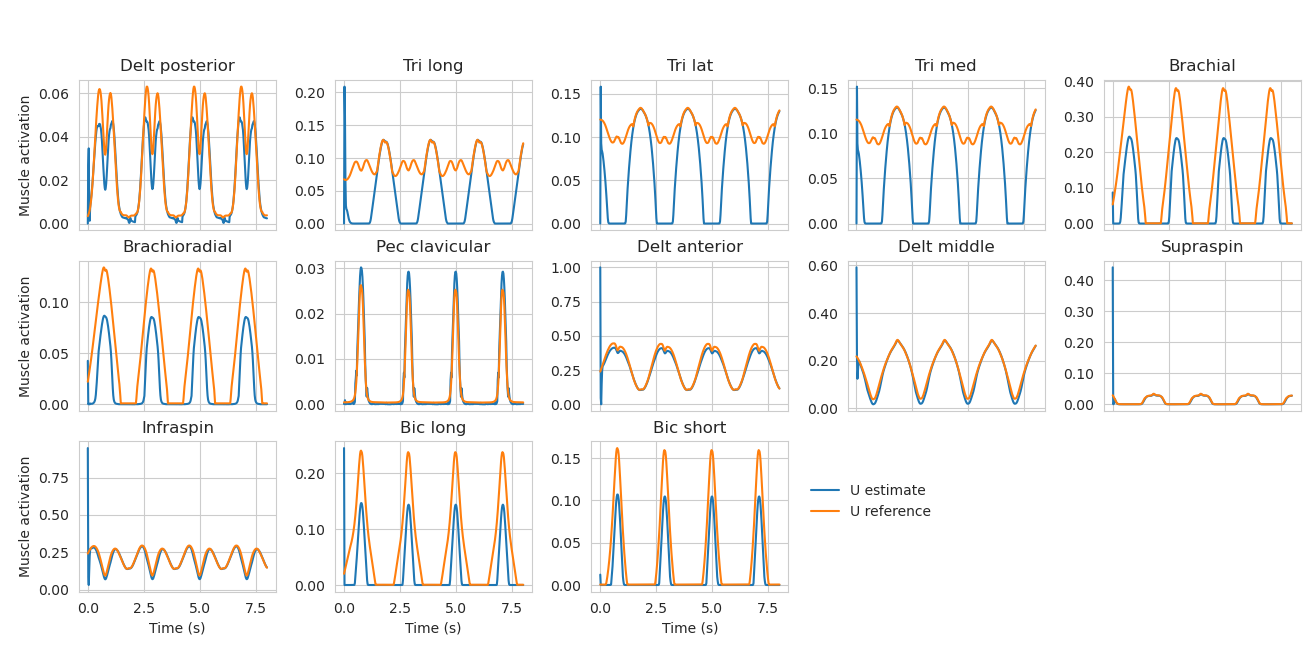
\includegraphics[width=\textwidth]{Muscles_excitations_MHE.png}\\ 
\caption{Time histories of estimate muscles activations (blue) and co-contracted muscles activations (orange) with significative action on motion (peaks activation level $>$ 0.1). 
Muscles' abbreviations stand for (from left to right and top to bottom): Triceps long head, lateral and medial, Brachial, Brachioradialis, Deltoid Anterior and Middle, Infraspinatus, Subscapularis, Biceps Brachial long and short head.} 
\label{fig:muscles_excitations_MHE} 
\end{figure*} 

